\documentclass[12pt,oneside]{abntex2}
\usepackage{mathptmx}
\usepackage[brazil]{babel}
\usepackage[utf8]{inputenc}
\usepackage[T1]{fontenc}
\usepackage{graphicx}
\usepackage{amsmath, amssymb}
\usepackage{lipsum}
\usepackage{setspace}
\usepackage{indentfirst}
\usepackage{setspace}
\usepackage{enumerate}
\usepackage{tocloft}
\usepackage{float}
\usepackage{hyperref}
\usepackage{geometry}
\geometry{a4paper, top=3cm, bottom=2cm, left=3cm, right=2cm}
\setcounter{section}{0} 
\renewcommand{\thesection}{\arabic{section}} 
\usepackage{placeins}
\usepackage{titlesec}

% Deixa todas as seções e subseções em 12pt (normalsize)
\titleformat{\section}{\normalsize\bfseries}{\thesection}{1em}{}
\titleformat{\subsection}{\normalsize\bfseries}{\thesubsection}{1em}{}
\titleformat{\subsubsection}{\normalsize\bfseries}{\thesubsubsection}{1em}{}

\usepackage[justification=justified, singlelinecheck=false]{caption}




\title{Análise Econômica do comportamento da Inflação entre o período de 2012 à 2025 em Regressão Linear}
\author{Nathan Pereira Gomes de Sousa \\ José João Victor De Oliveira Lima Almeida }
\date{18 de Setembro de 2025}
\local{Campina Grande - PB}
\instituicao{Universidade Federal de Campina Grande \\
Curso de Bacharelado em Ciências Econômicas}
\tipotrabalho{Atividade Avaliativa}

% Espaçamento 1,5
\OnehalfSpacing

\begin{document}

\begin{center}
{\textbf{\fontsize{14}{16}\selectfont 
UNIVERSIDADE FEDERAL DE CAMPINA GRANDE\\[1ex]
CENTRO DE HUMANIDADES\\[1ex]
UNIDADE ACADÊMICA DE ECONOMIA E FINANÇAS}}
\end{center}

% Capa
\imprimircapa

% Folha de rosto
\imprimirfolhaderosto*

% Sumário
\tableofcontents*
\newpage

\section{\textbf{Introdução}}

Esta atividade tem como objetivo aplicar conceitos de regressão linear para investigar o comportamento da inflação no Brasil, por meio da análise empírica da Curva de Phillips aceleracionista ou moderna com expectativas racionais.

O estudo da macroeconomia concentra-se na análise de variáveis que afetam o funcionamento da economia como um todo. Dentre essas variáveis, destacam-se os índices de inflação e as taxas de desemprego, que são alvo de constantes estudos, especialmente pela ligação observada entre elas. Um dos modelos teóricos mais relevantes nesse contexto é a Curva de Phillips, que sugere a existência de uma correlação negativa entre inflação e desemprego em determinados períodos históricos (BLANCHARD, 2001).

A lógica por trás dessa relação está associada ao comportamento das empresas e trabalhadores. Quando o nível de atividade econômica está aquecido e o desemprego está baixo, os salários tendem a subir, o que, por sua vez, pode pressionar os preços para cima, gerando inflação. Por outro lado, quando há alto desemprego, a demanda por bens e serviços enfraquece, os salários crescem mais lentamente e a inflação tende a diminuir (BLANCHARD, 2001).

\subsection*{\textbf{Teorias econômicas e evidências empíricas}}

A origem da Curva de Phillips remonta ao trabalho de A. W. Phillips (1958), que, ao analisar dados do Reino Unido entre 1861 e 1957, identificou uma relação inversa entre inflação e desemprego. Posteriormente, Samuelson e Solow (1960) confirmaram resultados semelhantes para os Estados Unidos, com dados de 1900 a 1960. Essa descoberta teve grande influência na formulação de políticas econômicas, pois indicava que governos poderiam escolher entre inflação baixa com desemprego alto ou inflação alta com desemprego baixo.  

Na década de 1970, porém, essa relação quebrou. Nos Estados Unidos, assim como na maioria dos países da OCDE, verificou-se inflação alta acompanhada de desemprego elevado, o que contradizia explicitamente a curva de Phillips original. Uma relação voltou a aparecer, mas sob a forma de associação entre a taxa de desemprego e a variação da taxa de inflação (Blanchard, 2001).  

Por que a curva de Phillips original desapareceu? Porque os fixadores de salários mudaram a forma de formar suas expectativas em relação à inflação. Essa mudança decorreu da própria transformação no comportamento da inflação: esta se tornou mais persistente, aumentando a probabilidade de que um ano de inflação alta fosse seguido por outro também elevado. Assim, os agentes passaram a levar em conta essa persistência ao formar suas expectativas. Essa alteração na formação de expectativas modificou a natureza da relação entre desemprego e inflação (Blanchard, 2001).  

Blanchard (2001) ressalta que a relação negativa prevista pela curva de Phillips é observada quando, no eixo horizontal, coloca-se a taxa de desemprego e, no eixo vertical, as variações da taxa de inflação. Nesse caso, a taxa de desemprego determina a aceleração da inflação.  

A formulação inicial da curva é dada por:

\[
\pi = (u - u_n)
\]

onde:
\begin{itemize}
    \item $\pi$ representa a inflação;
    \item $(u - u_n)$ representa a diferença entre o desemprego efetivo e o desemprego natural.
\end{itemize}

A diferença $(u - u_n)$ capta o desvio do desemprego em relação ao seu nível natural. Quando o desemprego efetivo $u$ está abaixo do desemprego natural $u_n$, a pressão sobre os preços tende a ser positiva, resultando em inflação. Por outro lado, quando o desemprego efetivo é superior ao nível natural, a pressão é negativa, indicando tendência de desaceleração inflacionária ou até deflação.  

Essa relação expressa o núcleo da Curva de Phillips, que sugere um trade-off de curto prazo entre inflação e desemprego. Entretanto, a experiência empírica mostrou que esse mecanismo não se mantinha estável ao longo do tempo, sobretudo quando a inflação passou a se tornar persistente.  

Enquanto a inflação permanecia relativamente baixa e pouco persistente, trabalhadores e empresas tendiam a assumir uma expectativa constante para a inflação futura, muitas vezes desconsiderando a inflação passada. Esse foi o contexto inicial observado, em que o desemprego $u$ girava em torno de níveis próximos ao natural e as expectativas eram praticamente fixas.  

Contudo, à medida que a inflação começou a se mostrar mais duradoura, especialmente a partir da década de 1970, trabalhadores e empresas passaram a ajustar suas expectativas com base na inflação passada. Nesse contexto, se a inflação tivesse sido elevada no período anterior, esperava-se que também fosse elevada no período seguinte. Esse processo levou à incorporação das expectativas na formulação da Curva de Phillips, resultando na chamada **Curva de Phillips aumentada pelas expectativas**:

\[
\pi = \pi^e - \phi (u_t - u_n)
\]

onde:
\begin{itemize}
    \item $\pi^e$: representa a inflação esperada;
    \item $\phi > 0$: é o parâmetro que mede a sensibilidade da inflação em relação ao desvio do desemprego.
\end{itemize}

Assim, a versão aumentada ou aceleracionista reconhece que não basta considerar apenas o hiato do desemprego, mas também a forma como os agentes formam expectativas sobre a inflação futura. Essa formulação indica que uma taxa de desemprego baixa leva a um aumento da taxa de inflação e, consequentemente, a uma aceleração do nível de preços. 

\subsection*{\textbf{Expectativas adaptativas e racionais}}

Uma vez que a expectativa de inflação influencia o trade-off entre inflação e desemprego no curto prazo, é crucial compreender como os agentes formam suas expectativas. Inicialmente, admite-se a hipótese de expectativas adaptativas, segundo a qual a inflação esperada depende da inflação recentemente observada. Nesse caso, trabalhadores e empresas ajustam suas previsões de forma gradual, levando em conta a inflação passada. Embora plausível, esse pressuposto é considerado simples demais para capturar todas as circunstâncias relevantes.

Uma abordagem alternativa e mais sofisticada é a das expectativas racionais. Nessa formulação, presume-se que os agentes fazem o melhor uso possível das informações disponíveis ao tomar decisões, incluindo dados sobre a condução das políticas monetária e fiscal. Assim, a inflação esperada $\pi_t^e$ não depende apenas do comportamento passado da inflação, mas também da credibilidade e do regime de política econômica vigente. Os erros do passado deixam de influir diretamente nas expectativas do presente, e os agentes não incorrem em erros sistemáticos, isto é, os erros de diferentes períodos não são autocorrelacionados.

Na versão fraca da hipótese de expectativas racionais, os agentes apenas utilizam todas as informações disponíveis, sem vínculos adicionais. Já na versão forte, assume-se que os agentes, em média, acertam o valor efetivo da variável. Formalmente:

\[
E(e_t) = 0 \quad \text{e} \quad \text{Cov}(e_t, e_{t-1}) = 0,
\]

em que $E$ denota a esperança matemática (média esperada), $\text{Cov}$ representa a covariância e $e_t$ é o erro de previsão.  

Assumir expectativas racionais traz implicações relevantes para a análise econômica. Considere, por exemplo, o caso em que os salários sejam fixos devido a contratos de trabalho. Se houver uma expansão monetária inesperada, a demanda agregada se desloca, elevando o nível de preços e reduzindo o salário real. Isso torna o trabalho mais barato, induzindo as empresas a contratar mais mão de obra, elevando o produto. Por outro lado, se a expansão monetária já era antecipada, trabalhadores e empresas podem incluir cláusulas de correção automática nos contratos, ajustando salários nominais. Nesse caso, a expansão da oferta monetária eleva simultaneamente demanda e oferta agregada, neutralizando os efeitos sobre emprego e produto.

Dessa forma, a Curva de Phillips com expectativas racionais pode ser expressa como:

\[
\pi_t = \pi_t^e - \phi (u_t - u_n) + v_t,
\]

onde:
\begin{itemize}
    \item $\pi_t$ é a inflação no período $t$;
    \item $\pi_t^e$ a inflação esperada;
    \item $u_t$ o desemprego efetivo;
    \item $u_n$ o desemprego natural;
    \item $\phi > 0$ mede a sensibilidade da inflação ao desvio do desemprego; 
    \item $v_t$ representa choques aleatórios.  
\end{itemize}

Como argumenta Sargent (2011), a persistência inflacionária observada não decorre de uma “força inercial” da inflação em si, mas das políticas econômicas que alimentam expectativas futuras. Dessa perspectiva, a inflação pode ser reduzida de forma mais rápida e menos custosa do que preveem modelos baseados em expectativas adaptativas, desde que a política adotada seja crível (Mankiw, 2011).  

Nessa hipótese, o trade-off de curto prazo desaparece, mostrando como a credibilidade da política econômica é central para a Curva de Phillips aumentada pelas expectativas.

\section{\textbf{Metodologia}}

A relação entre inflação e desemprego tem sido amplamente discutida na teoria macroeconômica, nesse estudo a partir da formulação da Curva de Phillips e a sua versão aceleracionista em que ela descreve uma interdependência negativa entre a variával explica inflação (IPCA) e a taxa de desemprego sugerindo que, em determinados contextos, taxas mais baixas de desemprego estão associadas a taxas mais altas de inflação, e vice-versa, assim como a variavel expectativa de inflação e a taxa básica de juros do Brasil entre 2012 e 2025.

As variáveis selecionadas foram: o Índice de Preço ao Consumidor Amplo (IPCA), utilizado para mensurar a inflação no Brasil; o nível de desemprego da economia brasileira, dessazonalizado pelo Instituto de Pesquisa Econômica Aplicada (IPEA); a taxa básica de juros over; o Índice de Confiança do Consumidor (ICC), disponibilizado pela Federação do Comércio do Estado de São Paulo (Fecomercio SP); e a expectativa de inflação do Boletim FOCUS, utilizada como proxy para a expectativa do mercado. O período considerado vai de janeiro de 2012 (01/2012) até maio de 2025 (05/2025).

A escolha dessas variáveis se fundamenta na relevância da Curva de Phillips, que sugere uma relação negativa entre desemprego e inflação em determinados contextos macroeconômicos, bem como na importância das expectativas de inflação para a dinâmica da economia.
O IPCA é o principal índice de inflação utilizado pelo Banco Central do Brasil para a formulação da política monetária, refletindo a variação de preços de uma cesta de bens e serviços consumidos pelas famílias com rendimentos entre 1 e 40 salários mínimos. Já a taxa de desemprego é um dos principais indicadores do mercado de trabalho, refletindo a proporção da força de trabalho que está desocupada e procurando emprego. Ambas as variáveis são fundamentais para a compreensão do comportamento da economia e são amplamente utilizadas na formulação de políticas econômicas.

\subsection{\textbf{Descrição e Coleta de Dados}}

Os dados utilizados neste trabalho foram obtidos a partir de três fontes principais: Instituto de Pesquisa Econômica Aplicada (IPEA), Sistema Gerenciador de Séries Temporais (SGS) e o Sistema de Expectativas de Mercado, ambos do Banco Central do Brasil. As séries foram selecionadas de acordo com a disponibilidade, relevância e consistência metodológica para a análise da Curva de Phillips no contexto brasileiro.

Para a inflação, foi considerado o Índice Nacional de Preços ao Consumidor Amplo (IPCA), série \texttt{PRECOS12\_IPCAG12}, disponibilizada pelo IBGE, cuja frequência é mensal. O IPCA mede a variação dos preços de uma cesta de bens e serviços representativa do consumo das famílias brasileiras, abrangendo rendimentos entre 1 e 40 salários mínimos e aproximadamente 90\% das famílias residentes em áreas urbanas cobertas pelo \textit{Sistema Nacional de Índices de Preços ao Consumidor} (SNIPC).

Para a taxa de desemprego, adotou-se a série \texttt{PNADC12\_TDESOCMD12}, obtida no IPEA, que corresponde à taxa de desocupação das pessoas de 14 anos ou mais de idade, mensalizada e dessazonalizada. Essa série é derivada da PNAD Contínua do IBGE, com ajustes metodológicos descritos na Nota Técnica nº 62 do IPEA, cobrindo o período de 2012.01 até 2025.05. A dessazonalização foi realizada pelo método X-13 ARIMA, sem ajustes para feriados móveis ou \textit{outliers}.

O Índice de Confiança do Consumidor (ICC), disponibilizado pela Federação do Comércio do Estado de São Paulo (Fecomercio SP), também foi incluído. O ICC mede o sentimento dos consumidores em relação às suas condições econômicas atuais e expectativas futuras, sendo construído a partir de questionários que captam diferenças entre respostas positivas e negativas. O índice varia de 0 (pessimismo total) a 200 (otimismo total) e desdobra-se em dois componentes: o Índice de Condições Econômicas Atuais (ICEA) e o Índice de Expectativas do Consumidor (IEC).

Adicionalmente, incluiu-se a taxa de juros de referência, a Selic, série \texttt{BM12\_TJOVER12}, disponibilizada pelo Banco Central do Brasil. Trata-se da taxa de juros \textit{Over/Selic} acumulada no mês, calculada a partir das operações de um dia entre instituições financeiras, garantidas por títulos públicos, registrada no Sistema Selic.

Além das variáveis efetivas de inflação (IPCA), desemprego (PNAD Contínua/IPEA), confiança do consumidor (ICC) e taxa de juros (Selic), este trabalho também incorpora as expectativas de inflação extraídas do \textit{Sistema de Expectativas de Mercado} do Banco Central do Brasil. Essas expectativas resultam do acompanhamento contínuo das projeções feitas por instituições financeiras, consultorias e demais agentes de mercado, sendo consolidadas no Boletim Focus. O uso das expectativas de inflação tem como objetivo captar a dimensão prospectiva do comportamento dos agentes econômicos, refletindo como estes formam suas previsões sobre a dinâmica futura dos preços. Tal variável pode ser considerada uma \textit{proxy} para a inflação esperada, dado que não é observada diretamente na economia, mas inferida a partir de informações coletadas pelo Banco Central.

Assim, a inclusão dessa medida é coerente com a literatura macroeconômica que ressalta o papel central das expectativas na determinação da inflação e na formulação da política monetária. Ao controlar para a inflação esperada, busca-se avaliar se a relação entre inflação observada e desemprego mantém-se consistente com a Curva de Phillips ou se passa a depender fortemente das expectativas dos agentes.

\medskip

O período de análise considerado neste estudo vai de janeiro de 2012 (01/2012) até maio de 2025 (05/2025), respeitando a interseção temporal entre as séries. Após a coleta, os dados foram tratados no software estatístico R: as séries foram convertidas para o formato de data adequado, inspecionadas quanto à presença de valores faltantes, harmonizadas em frequência e unificadas em um único \textit{dataframe}. Foram realizadas análises descritivas e gráficas, bem como estimativas econométricas (regressão linear), com o objetivo de investigar empiricamente a relação entre inflação e desemprego e avaliar a validade da Curva de Phillips no caso brasileiro.

\medskip
\noindent \textbf{Fontes:} \\
Instituto de Pesquisa Econômica Aplicada (IPEA) – Taxa de desocupação; \\
Instituto Brasileiro de Geografia e Estatística (IBGE/SNIPC) – IPCA; \\
Banco Central do Brasil (BACEN) – Taxa Selic; \\
Banco Central do Brasil – Sistema de Expectativas de Mercado – Expectativas de inflação; \\
Federação do Comércio do Estado de São Paulo (Fecomercio SP) – Índice de Confiança do Consumidor. \\

\textbf{Período:} Mensal, de janeiro de 2012 (01/2012) a maio de 2025 (05/2025).
\medskip

\subsection{\textbf{Modelo}}

Para a análise empírica, será empregada a regressão linear múltipla, ferramenta estatística fundamental para investigar a relação entre uma variável dependente e múltiplas variáveis explicativas. No presente estudo, considera-se a taxa de inflação (IPCA) como variável dependente, enquanto a taxa de desemprego (PNAD Contínua/IPEA), a taxa básica de juros (Selic Over), as expectativas de inflação (Boletim Focus) e o Índice de Confiança do Consumidor (ICC) são utilizadas como variáveis independentes. Dessa forma, pretende-se avaliar em que medida essas variáveis ajudam a compreender a dinâmica da inflação e verificar a aplicabilidade empírica da Curva de Phillips no Brasil. 

O modelo de regressão linear múltipla é representado pela seguinte equação geral:

\[
y = \alpha + \beta_1 x_1 + \beta_2 x_2 + \beta_3 x_3 + \beta_4 x_4 + \varepsilon_i
\]

onde:
\begin{itemize}
    \item $y$ representa a variável dependente, a inflação (IPCA);
    \item $x_1 = \log(\text{Txdesocup})$, o logaritmo da taxa de desemprego;
    \item $x_2 = \log(\text{SelicOver})$, o logaritmo da taxa básica de juros mensal;
    \item $x_3 = \text{ExpIPCA}$, as expectativas de inflação do mercado (Boletim Focus);
    \item $x_4 = \text{ICC}$, o Índice de Confiança do Consumidor;
    \item $\alpha$ é o intercepto do modelo, indicando o valor esperado de $y$ quando todas as variáveis independentes assumem valor zero;
    \item $\beta_i$ são os coeficientes angulares, que representam a variação esperada em $y$ para cada unidade de variação em $x_i$, mantendo as demais variáveis constantes;
    \item $\varepsilon_i$ é o termo de erro, que captura os efeitos de outras variáveis não incluídas no modelo.
\end{itemize}

A transformação logarítmica foi aplicada às variáveis taxa de desemprego e taxa de juros (Selic Over) por duas razões principais:  
(i) reduzir a assimetria da distribuição dessas séries, aproximando-as de uma forma mais próxima da normalidade, condição desejável para os pressupostos da regressão linear; e  
(ii) permitir a interpretação dos coeficientes estimados em termos aproximados de elasticidades, ou seja, variações percentuais na inflação (IPCA) em resposta a variações percentuais nessas variáveis.

A escolha por esse tipo de regressão se justifica por sua simplicidade, interpretabilidade e ampla aplicação em análises econômicas. Além disso, permite verificar se há uma associação estatisticamente significativa entre desemprego e inflação, bem como o papel das expectativas e da confiança do consumidor, contribuindo para a compreensão da dinâmica inflacionária brasileira e da aplicabilidade empírica da Curva de Phillips.

\section{\textbf{Análise dos Resultados}}

\subsection{\textbf{Modelo de Regressão}}

Para investigar empiricamente a Curva de Phillips no Brasil, foi estimada uma regressão linear múltipla com a inflação medida pelo IPCA como variável dependente e quatro variáveis explicativas: taxa de desemprego (logaritmo da taxa dessazonalizada), taxa básica de juros Selic Over (logaritmo), expectativa de inflação do Boletim Focus (proxy para inflação esperada) e o Índice de Confiança do Consumidor (ICC). 

O uso do logaritmo natural nas variáveis desemprego e taxa de juros tem como objetivo reduzir a variabilidade, estabilizar a variância e permitir uma interpretação em termos de elasticidade, isto é, variações proporcionais na inflação em resposta a variações proporcionais nessas variáveis. 

O modelo estimado pode ser representado pela seguinte equação:

\[
IPCA_t = \alpha + \beta_1 \cdot \log(TxDesocup_t) + \beta_2 \cdot \log(SelicOver_t) + \beta_3 \cdot ExpIPCA_t + \beta_4 \cdot ICC_t + \varepsilon_t
\]

Substituindo pelos coeficientes estimados, obtém-se:

\[
IPCA_t = 0.680085 \;-\; 0.228331 \cdot \log(TxDesocup_t) \;-\; 0.424623 \cdot \log(SelicOver_t) \;+\; 1.386442 \cdot ExpIPCA_t \;-\; 0.030011 \cdot ICC_t \;+\; \varepsilon_t
\]

\begin{table}[H]
\centering
\caption{Resultados da Regressão Linear Múltipla – Variável Dependente: IPCA}
\begin{tabular}{lcccc}
\hline
Variável & Coeficiente & Erro Padrão & Estatística t & p-Valor \\
\hline
LOG\_TXDESOCUP & -0.228331 & 0.107463 & -2.124734 & 0.0352 \\
LOG\_SELIC     & -0.424623 & 0.050168 & -8.467902 & 0.0000 \\
EXPIPCA        &  1.386442 & 0.088768 & 15.58322  & 0.0000 \\
ICC            & -0.030011 & 0.012055 & -2.489634 & 0.0140 \\
C (Constante)  &  0.680085 & 0.349353 &  1.946640 & 0.0543 \\
\hline
\multicolumn{5}{c}{\textbf{Estatísticas do Modelo}} \\
\hline
R-quadrado             & \multicolumn{4}{c}{0.620534} \\
R-quadrado ajustado    & \multicolumn{4}{c}{0.610804} \\
Erro padrão da regressão & \multicolumn{4}{c}{0.231154} \\
Soma dos quadrados dos resíduos & \multicolumn{4}{c}{8.521496} \\
Log-likelihood         & \multicolumn{4}{c}{8.522496} \\
Estatística F          & \multicolumn{4}{c}{63.77596 (p=0.0000)} \\
Durbin-Watson          & \multicolumn{4}{c}{1.846278} \\
\hline
\end{tabular}
\end{table}

A interpretação dos coeficientes estimados revela aspectos importantes da dinâmica entre as variáveis escolhidas e a inflação (IPCA). O coeficiente da taxa de desemprego ($\log(\text{Txdesocup})$) apresentou sinal negativo, em linha com a Curva de Phillips, indicando que um aumento no desemprego está associado a uma redução da inflação. Já a taxa de juros básica ($\log(\text{Selic})$) também apresentou sinal negativo, como esperado, reforçando o papel da política monetária contracionista na contenção dos preços. As expectativas de inflação (ExpIPCA) mostraram coeficiente positivo e elevado, sugerindo que as percepções do mercado têm efeito significativo e direto sobre a formação da inflação corrente, confirmando a importância das expectativas racionais no processo inflacionário.

O Índice de Confiança do Consumidor (ICC), por sua vez, apresentou coeficiente negativo, em aparente contradição à intuição inicial de que maior confiança elevaria a demanda e, portanto, a inflação. Contudo, esse resultado pode ser explicado por, o caráter do ICC como indicador de sentimento econômico, que tende a cair em momentos de alta inflação, refletindo mais a percepção de estabilidade macroeconômica do que um impulso inflacionário. Assim, o sinal negativo sugere que, no período analisado, maior confiança refletiu expectativas de estabilidade e controle inflacionário, e não pressões adicionais de demanda.

Portanto, a interpretação dos coeficientes mostra consistência com a teoria econômica nos principais determinantes (desemprego, juros e expectativas), ao mesmo tempo em que revela a especificidade do comportamento do ICC no contexto brasileiro.

\subsection{\textbf{Teste de Heterocedasticidade de White}}

O teste de White é utilizado para verificar a presença de heterocedasticidade, ou seja, variância não constante dos resíduos. A hipótese nula do teste é a de homocedasticidade, isto é:

\[
H_0: \ \text{Os resíduos possuem variância constante (homocedasticidade).}
\]

\[
H_1: \ \text{Os resíduos apresentam heterocedasticidade.}
\]

No modelo estimado, o p-valor associado ao teste de White foi igual a 0.6414, indicando que não se rejeita a hipótese nula de homocedasticidade. Assim, conclui-se que não há evidências de heterocedasticidade nos resíduos. 

\begin{table}[H]
\centering
\caption{Resultado do Teste de Heterocedasticidade de White}
\begin{tabular}{lcc}
\hline
Estatística & Valor & p-Valor \\
\hline
F-statistic & -- & 0.6414 \\
Obs*R-squared & -- & 0.6224 \\
Scaled explained SS & -- & 0.0226 \\
\hline
\end{tabular}
\end{table}

Como não foi detectada heterocedasticidade, não houve necessidade de reestimar o modelo com a matriz de covariância robusta de White. 

\subsection{\textbf{Teste de Autocorrelação de Durbin-Watson}}

O teste de Durbin-Watson (DW) é utilizado para verificar autocorrelação de primeira ordem nos resíduos. 
A hipótese nula é de ausência de autocorrelação:

\[
H_0: \ \text{Não há autocorrelação de primeira ordem nos resíduos.}
\]

No modelo estimado, o valor da estatística de Durbin-Watson foi 1.846, próximo de 2, o que sugere ausência de autocorrelação significativa.

\begin{table}[H]
\centering
\caption{Resultado do Teste de Durbin-Watson}
\begin{tabular}{lc}
\hline
Estatística & Valor \\
\hline
Durbin-Watson & 1.846 \\
\hline
\end{tabular}
\end{table}

\subsection{\textbf{Teste LM (Breusch-Godfrey) para Autocorrelação}}

Como complemento, foi realizado o teste LM de Breusch-Godfrey para uma defasagem (lag 1). Este teste é mais geral que o Durbin-Watson, permitindo detectar autocorrelação de ordens superiores.

A hipótese nula é:
\[
H_0: \ \text{Não há autocorrelação nos resíduos.}
\]

Os resultados são apresentados na Tabela a seguir:

\begin{table}[H]
\centering
\caption{Resultado do Teste LM (Breusch-Godfrey) com 1 defasagem}
\begin{tabular}{lcc}
\hline
Estatística & p-Valor \\
\hline
F-statistic & 0.3228 \\
Obs*R-squared & 0.3146 \\
\hline
\end{tabular}
\end{table}

Como os p-valores são superiores a 0,05, não se rejeita a hipótese nula. Conclui-se que não há evidências de autocorrelação nos resíduos, confirmando os resultados do teste de Durbin-Watson.



\subsection{\textbf{Gráficos para série de dados}}

A Figura 1 a seguir compara a evolução do IPCA observado com as expectativas de inflação do mercado. Nota-se que, embora as expectativas acompanhem de perto a trajetória da inflação efetiva, em alguns períodos há divergências relevantes, refletindo incertezas ou choques não antecipados pelos agentes econômicos. Essa diferença é importante, pois ilustra o papel das expectativas na dinâmica da inflação e justifica a sua inclusão como variável explicativa no modelo estimado.

\begin{figure}[htbp]
    \centering
    \caption{Inflação Observada vs Expectativas de Inflação}
    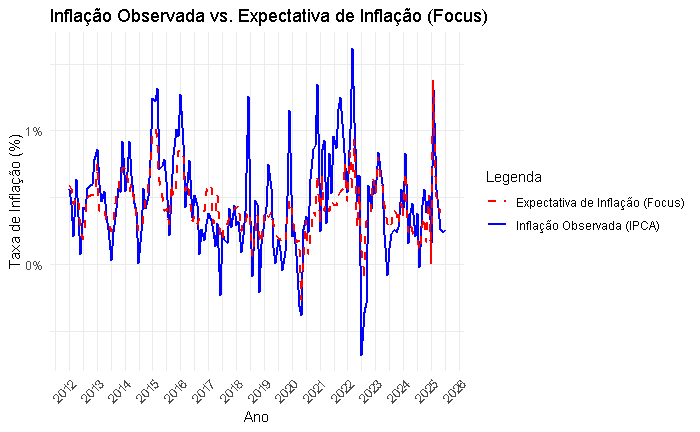
\includegraphics[width=0.8\textwidth]{IPCAxExp.png}
    \label{fig:IPCA-ExpIPCA}
     \legend{\footnotesize Fonte: Elaboração própria, a partir dos dados do SGS e Sistema Expectativas de mercado.}
\end{figure}


Na Figura 2, a trajetória da inflação observada é comparada com os valores ajustados pela regressão linear múltipla proposta. Observa-se que o modelo é capaz de reproduzir, em linhas gerais, a tendência do IPCA ao longo do tempo, ainda que apresente desvios em determinados momentos de maior volatilidade. Essa comparação fornece evidências de que as variáveis explicativas selecionadas (desemprego, taxa Selic, expectativas e ICC) conseguem capturar parte significativa da dinâmica inflacionária, mas também revela que choques específicos ou fatores não incluídos no modelo podem influenciar o comportamento dos preços.

\begin{figure}[htbp]
    \centering
    \caption{Inflação Observada vs Valores Ajustados pelo Modelo}
    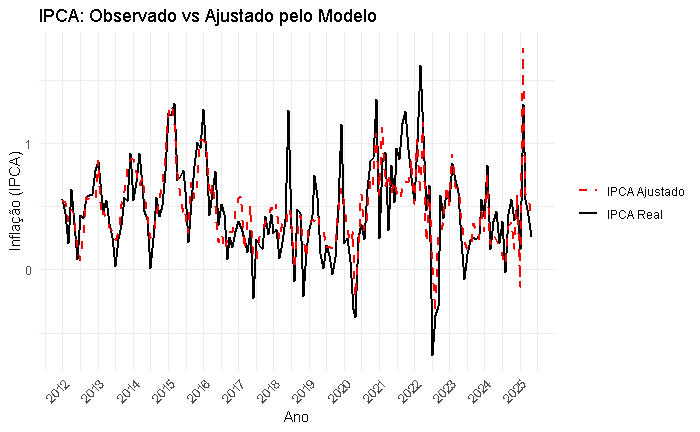
\includegraphics[width=0.8\textwidth]{IPCAxModelo.png}
    \label{fig:IPCA-ExpIPCA}
    \legend{\footnotesize Fonte: Elaboração própria.}
\end{figure}

\section{\textbf{Conclusão}}

Os sinais esperados dos coeficientes, segundo a teoria, indicavam que o desemprego e a taxa de juros deveriam apresentar relação negativa com a inflação, enquanto as expectativas inflacionárias e o índice de confiança do consumidor tenderiam a apresentar relação positiva. Os resultados confirmaram em grande parte essas expectativas, com exceção do ICC, que apresentou sinal contrário, sugerindo que, no contextos do Brasil, maior confiança pode estar associada à estabilidade de preços. 

Os testes de diagnóstico reforçaram a adequação do modelo, não foram encontrados indícios de heterocedasticidade ou autocorrelação dos resíduos, o que sustenta a validade estatística da estimação. Assim, o modelo mostrou-se consistente com a teoria econômica para a maior parte das variáveis analisadas, destacando o papel central do desemprego, da taxa de juros e das expectativas na determinação da inflação no Brasil, ainda que reste espaço para estudos adicionais acerca da influência da confiança do consumidor.


\section{\textbf{Referências bibliográficas}}
\setlength{\parindent}{0pt} % Remove o recuo da primeira linha
\setlength{\itemindent}{0pt} % Garante alinhamento
\setlength{\leftskip}{0pt}   % Garant



BACHA, Carlos José Caetano; LIMA, Roberto Arruda de Souza. \textbf{A curva de Phillips: teoria, evidência empírica e aplicabilidade à economia brasileira}. \textit{Pesquisa e Debate}, São Paulo, v. 15, n. 1(25), p. 131–162, 2004.



BANCO CENTRAL DO BRASIL. \textbf{Sistema Gerenciador de Séries Temporais – SGS.} Disponível em: \url{https://www3.bcb.gov.br/sgspub}. Acesso em: 27 ago. 2025.



BLANCHARD, Olivier. \textbf{\textit{Macroeconomia}}. 3. ed. São Paulo: Pearson, 2001.



GUJARATI, Damodar N. \textbf{\textit{Econometria básica}}. 4. ed. Rio de Janeiro: Elsevier, 2006.



IPEA — Instituto de Pesquisa Econômica Aplicada. \textbf{Ipeadata.} Disponível em: \url{https://ipeadata.gov.br/Default.aspx}. Acesso em: 27 ago. 2025.



MANKIW, N. Gregory. \textbf{\textit{Introdução à economia}}. 7. ed. São Paulo: Cengage Learning, 2021.



\end{document}
